%%%%%%%%%%%%%%%%%%%%%%%%%%%%%%%%%%%%%%%%%%%%%%%%%%%%%%%%%%%%%%%%%%%%%%%%%%%%%%%%%%%%%%%%%%%%%%%%%%%%%%%%%%%%%%
%                                                                                                            
%
% ------------------------------------------------------------------------------------------------------------ 
%  @desc        Diploma Thesis Digital Capnometer Module
% ------------------------------------------------------------------------------------------------------------
%               Written by Bastian Großauer
%
%               Feel free to add me in your "Danksagung" :)
%
% @authors      Bastian Großauer 
% 
% @datum        14.01.2022
% @file         DA.tex
%
% @depend       DA_1-4_CAPNO_nf.pdf --------------------------------------------------------------------------
%               DA_5-6_CAPNO_nf.pdf --------------------------------------------------------------------------
%               DA_7-8_CAPNO_nf.pdf --------------------------------------------------------------------------
%
% @comment      Diverse functions and packages only in LuaLaTex available
%               Therfore compile in LuaLaTeX ONLY!!!
%
%
%%%%%%%%%%%%%%%%%%%%%%%%%%%%%%%%%%%%%%%%%%%%%%%%%%%%%%%%%%%%%%%%%%%%%%%%%%%%%%%%%%%%%%%%%%%%%%%%%%%%%%%%%%%%%%               


\documentclass[12pt]{article}

%%%%%%%%%%%%%%%%%%%%%%%%%%%%%%%%%%%%%%%%%%%%%%%%%%% imports %%%%%%%%%%%%%%%%%%%%%%%%%%%%%%%%%%%%%%%%%%%%%%%%%%%

\usepackage{lingmacros}
\usepackage{tree-dvips}
\usepackage[utf8]{inputenc}
\usepackage{fontspec}
\usepackage{graphicx}
\usepackage{parskip}
\usepackage{xcolor}  
\usepackage{tocloft}
\usepackage{tabto}   
\usepackage{comment} 
\usepackage{pdfpages} 
\usepackage{fixltx2e}
\usepackage[12pt]{moresize}
\usepackage{lipsum}
\usepackage{titlesec}
\usepackage{titling}
\usepackage{geometry}
\geometry{
    twoside,
    a4paper,
    total={155mm,235mm},                                                                    % used text area
    left=35mm,                                                                              % explanation: https://www.overleaf.com/learn/latex/Page_size_and_margins
    top=30mm,   
}  
\usepackage{fancyhdr}
\usepackage[hyphens]{url}
\usepackage{hyperref}
\usepackage[style=ieee]{biblatex}                                                           %Imports biblatex package witg numeric citations instead of alphabetic
\usepackage[font=small, font=itshape,begintext=\textquotedblleft,endtext=\textquotedblright]{quoting} % set the \quote to italc and small
\usepackage{listings}
\usepackage{afterpage}                                                                      % Page Setup



\newcommand{\para}[1]{\paragraph{#1}\mbox{}}                                                % Paragraphs start below 
\newcommand{\subpara}[1]{\subparagraph{#1}\mbox{}}


\tolerance=1                                                                                % reduce word cuts at end of line
\emergencystretch=\maxdimen
\hyphenpenalty=10000
\hbadness=10000

\setlength{\headsep}{1.5cm}                                                                 % set spce between header and section
%\setlength{\parskip}{0.25cm}
%\setlength{\parindent}{0em}


% %%%%%%%%%%%%%%%%%%%%%%%%%%%%%%%%%%%%%%%%%%%% Code Listings Setup %%%%%%%%%%%%%%%%%%%%%%%%%%%%%%%%%%%%%%%%%%%





% %%%%%%%%%%%%%%%%%%%%%%%%%%%%%%%%%%%%%% Page and Header/Footer Setup %%%%%%%%%%%%%%%%%%%%%%%%%%%%%%%%%%%%%%%%


\pagestyle{fancy}                                                                           % Use fancyhdr as pagestyle
\fancyhead{}                                                                                % Reset Footer and Header once
\fancyfoot{}
 	
\setmainfont{Arial}                                                                         % Set Font to Arial (LuaLaTeX)

\setcounter{secnumdepth}{4}                                                                 % ??
\setcounter{tocdepth}{4}
\setcounter{secnumdepth}{5}
\setcounter{tocdepth}{5}


\renewcommand{\footrulewidth}{1pt}                                                          % Set Foot&Headline to 1pt
\renewcommand{\headrulewidth}{1pt}

\titlespacing\section{0pt}{12pt plus 4pt minus 2pt}{6pt plus 2pt minus 2pt}                 % Set Section Margins & Distances
\titlespacing\subsection{0pt}{12pt plus 4pt minus 2pt}{6pt plus 2pt minus 2pt}
\titlespacing\subsubsection{0pt}{12pt plus 4pt minus 2pt}{6pt plus 2pt minus 2pt}

\setlength{\cftsecindent}{1em}                                                              % Set Indents of in ToC
\setlength{\cftsubsecindent}{2em}
\setlength{\cftsubsubsecindent}{3em}
\setlength{\cftparaindent}{4em}
\setlength{\cftsubparaindent}{5em}

\addbibresource{references.bib}                                                             % Import the bibliography file




%%%%%%%%%%%%%%%%%%%%%%%%%%%%%%%%%%%%%%%%%%%%% Begin of Document %%%%%%%%%%%%%%%%%%%%%%%%%%%%%%%%%%%%%%%%%%%%%

\begin{document}



\makeatletter
\renewcommand\listoffigures{                                                                % Removes Header from List of Figures
        \@starttoc{lof}
}
\renewcommand\listoftables{                                                                 % Removes Header from List of tables
        \@starttoc{lot}
}
\renewcommand\lstlistoflistings{                                                            % Removes Header from Codelistings
        \@starttoc{lol}
}
\makeatother


%                                                                                           % not sure if there should by 1 blank or 2 in 1-4
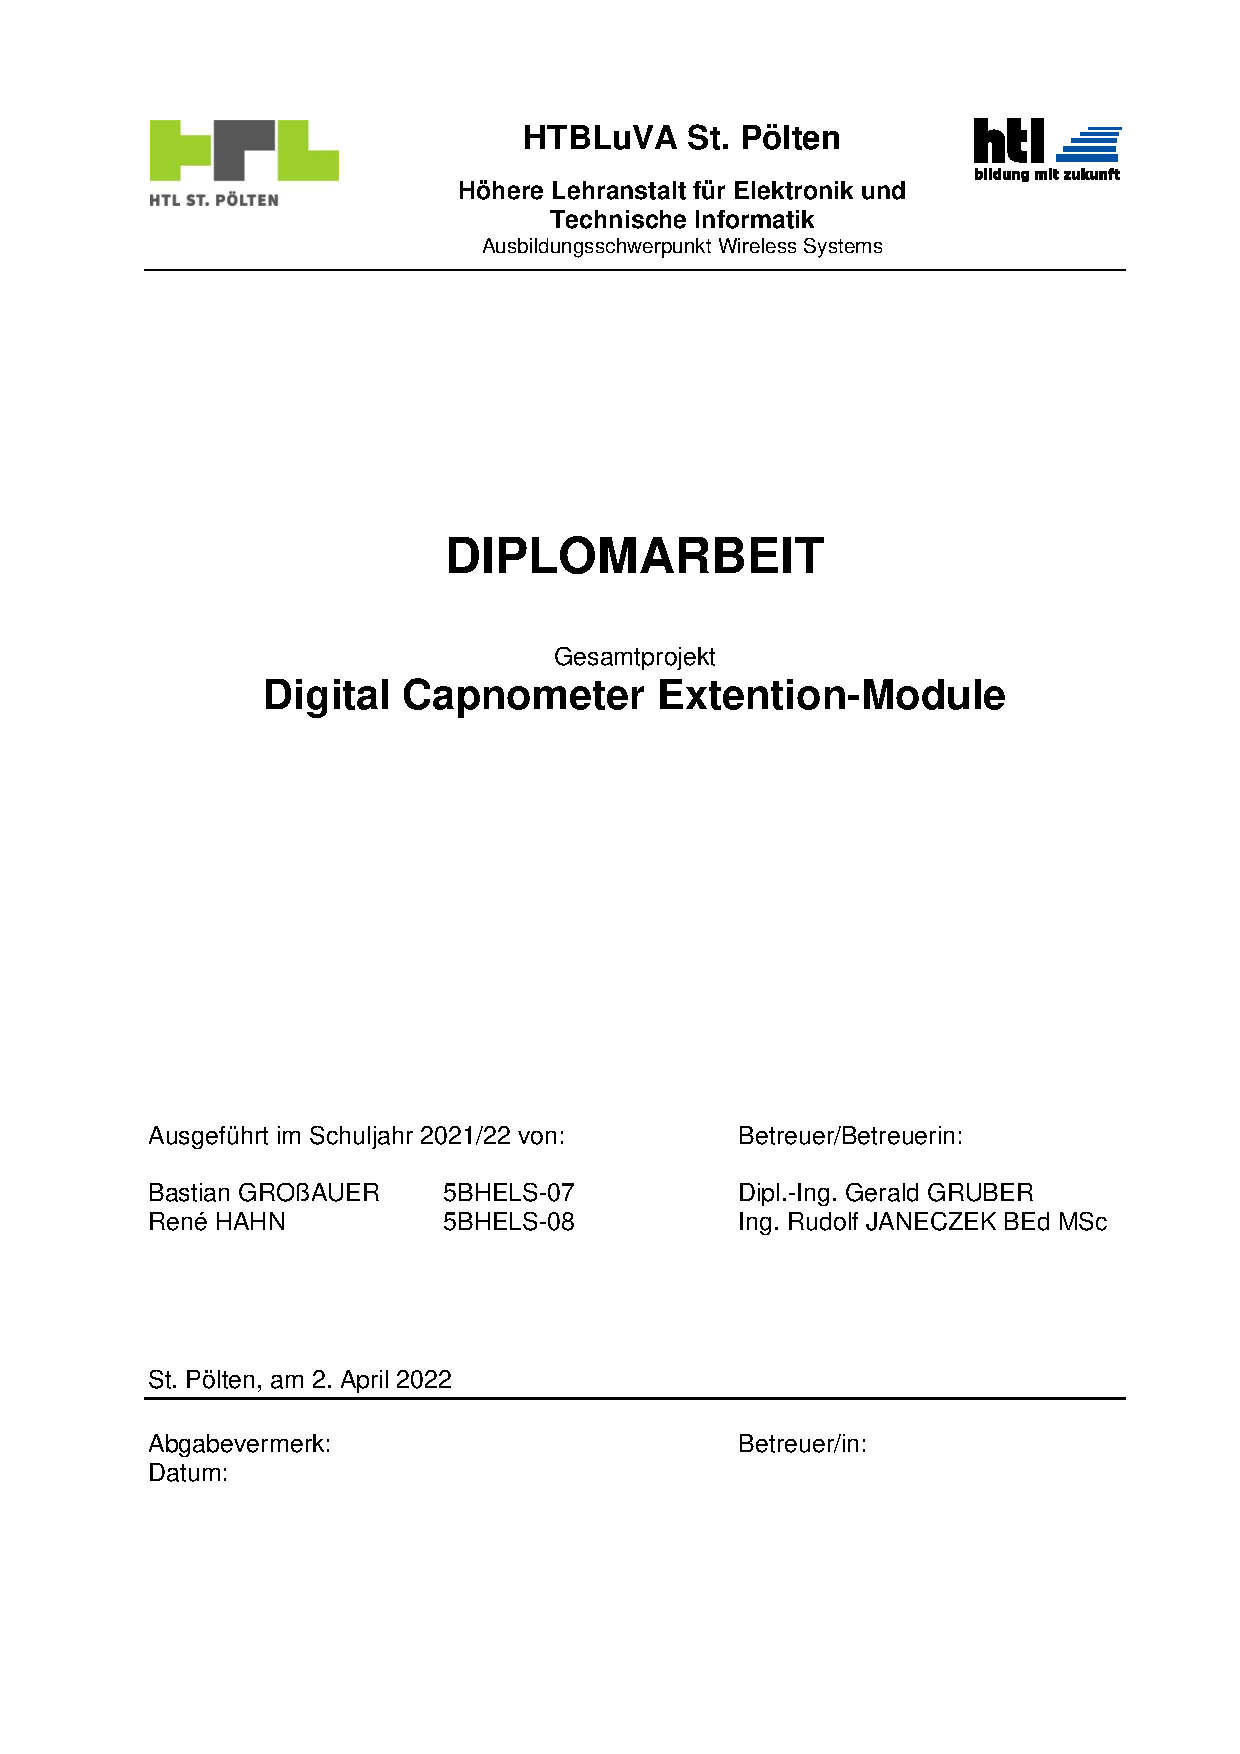
\includepdf[pages={1-3}]{./pdf/DA_1_CAPNO_nf.pdf}                                           % write the initial Document with the 
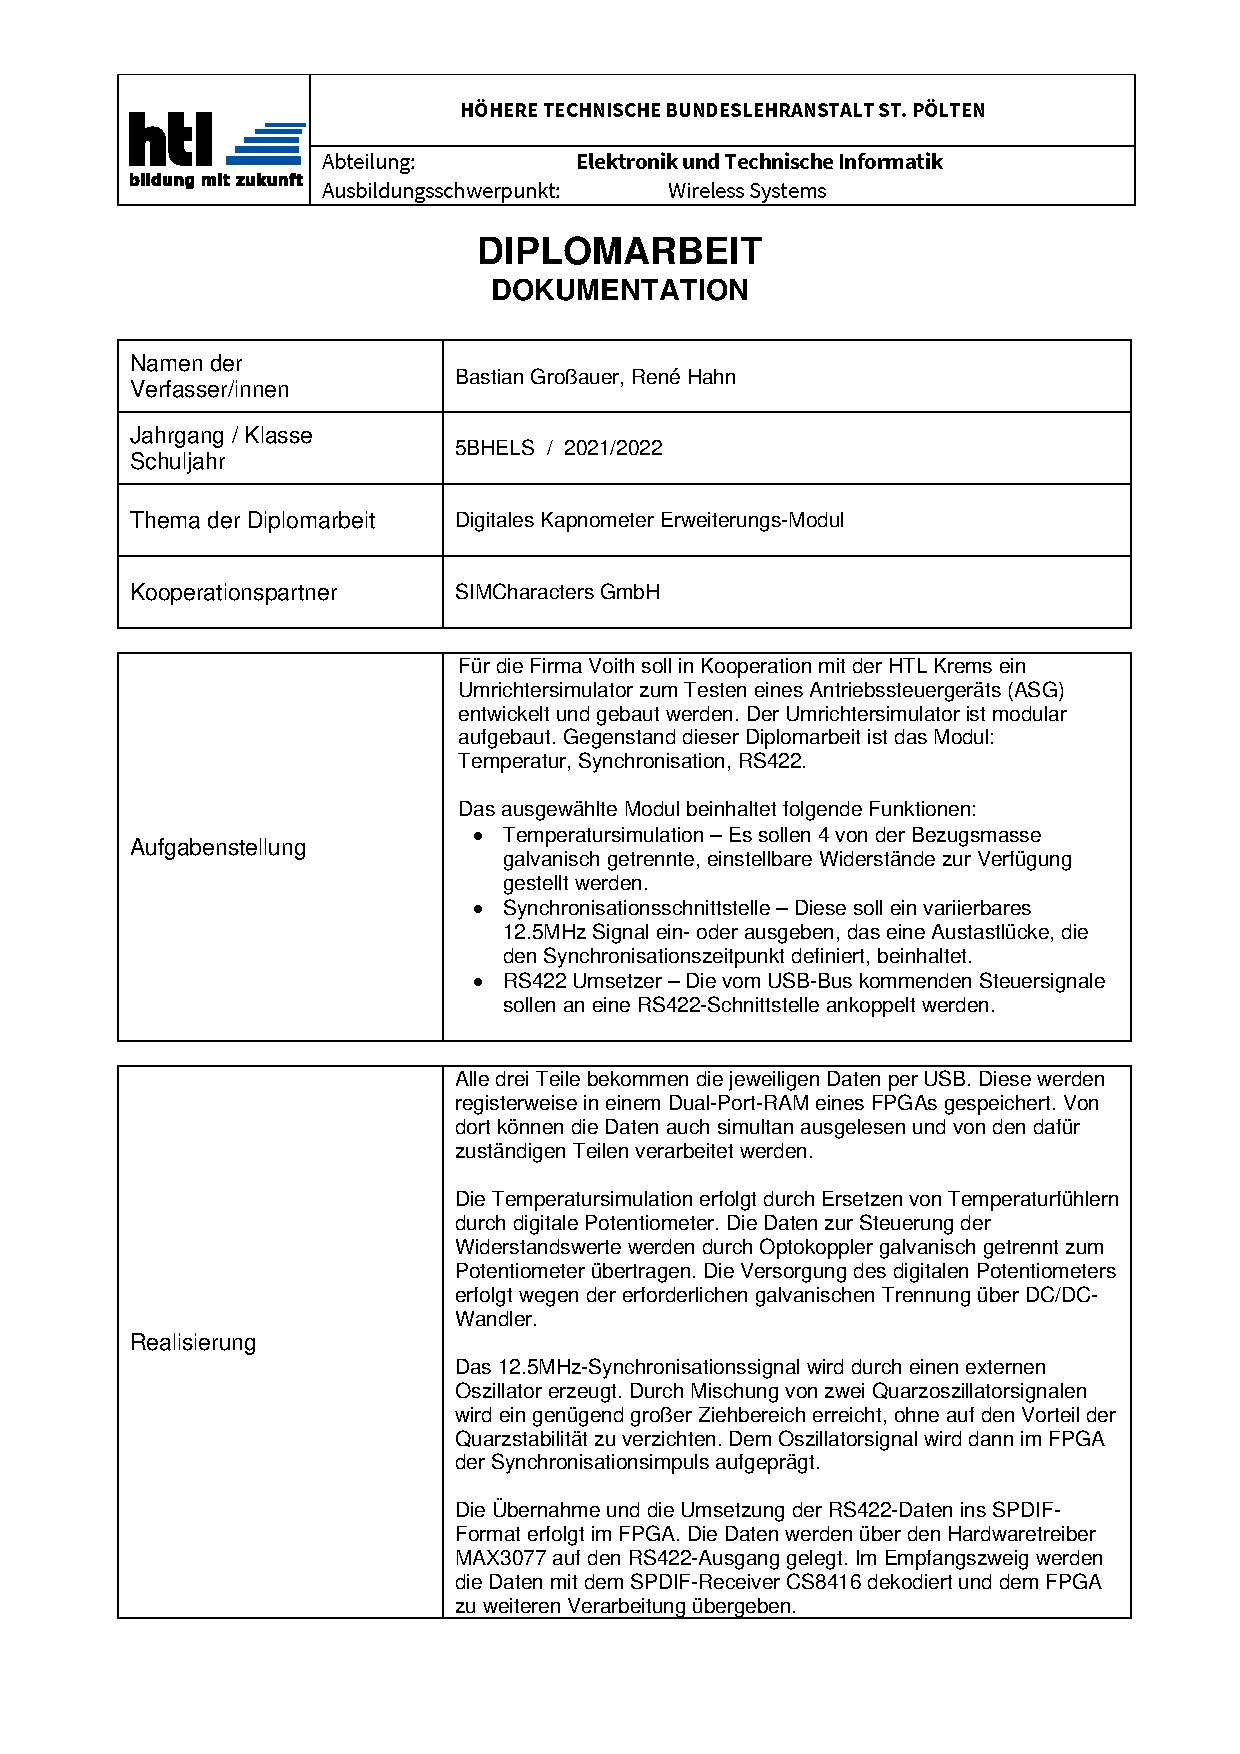
\includepdf[pages={1-2}]{./pdf/DA_2_CAPNO_nf.pdf}                                           % provided templates from sharepoint
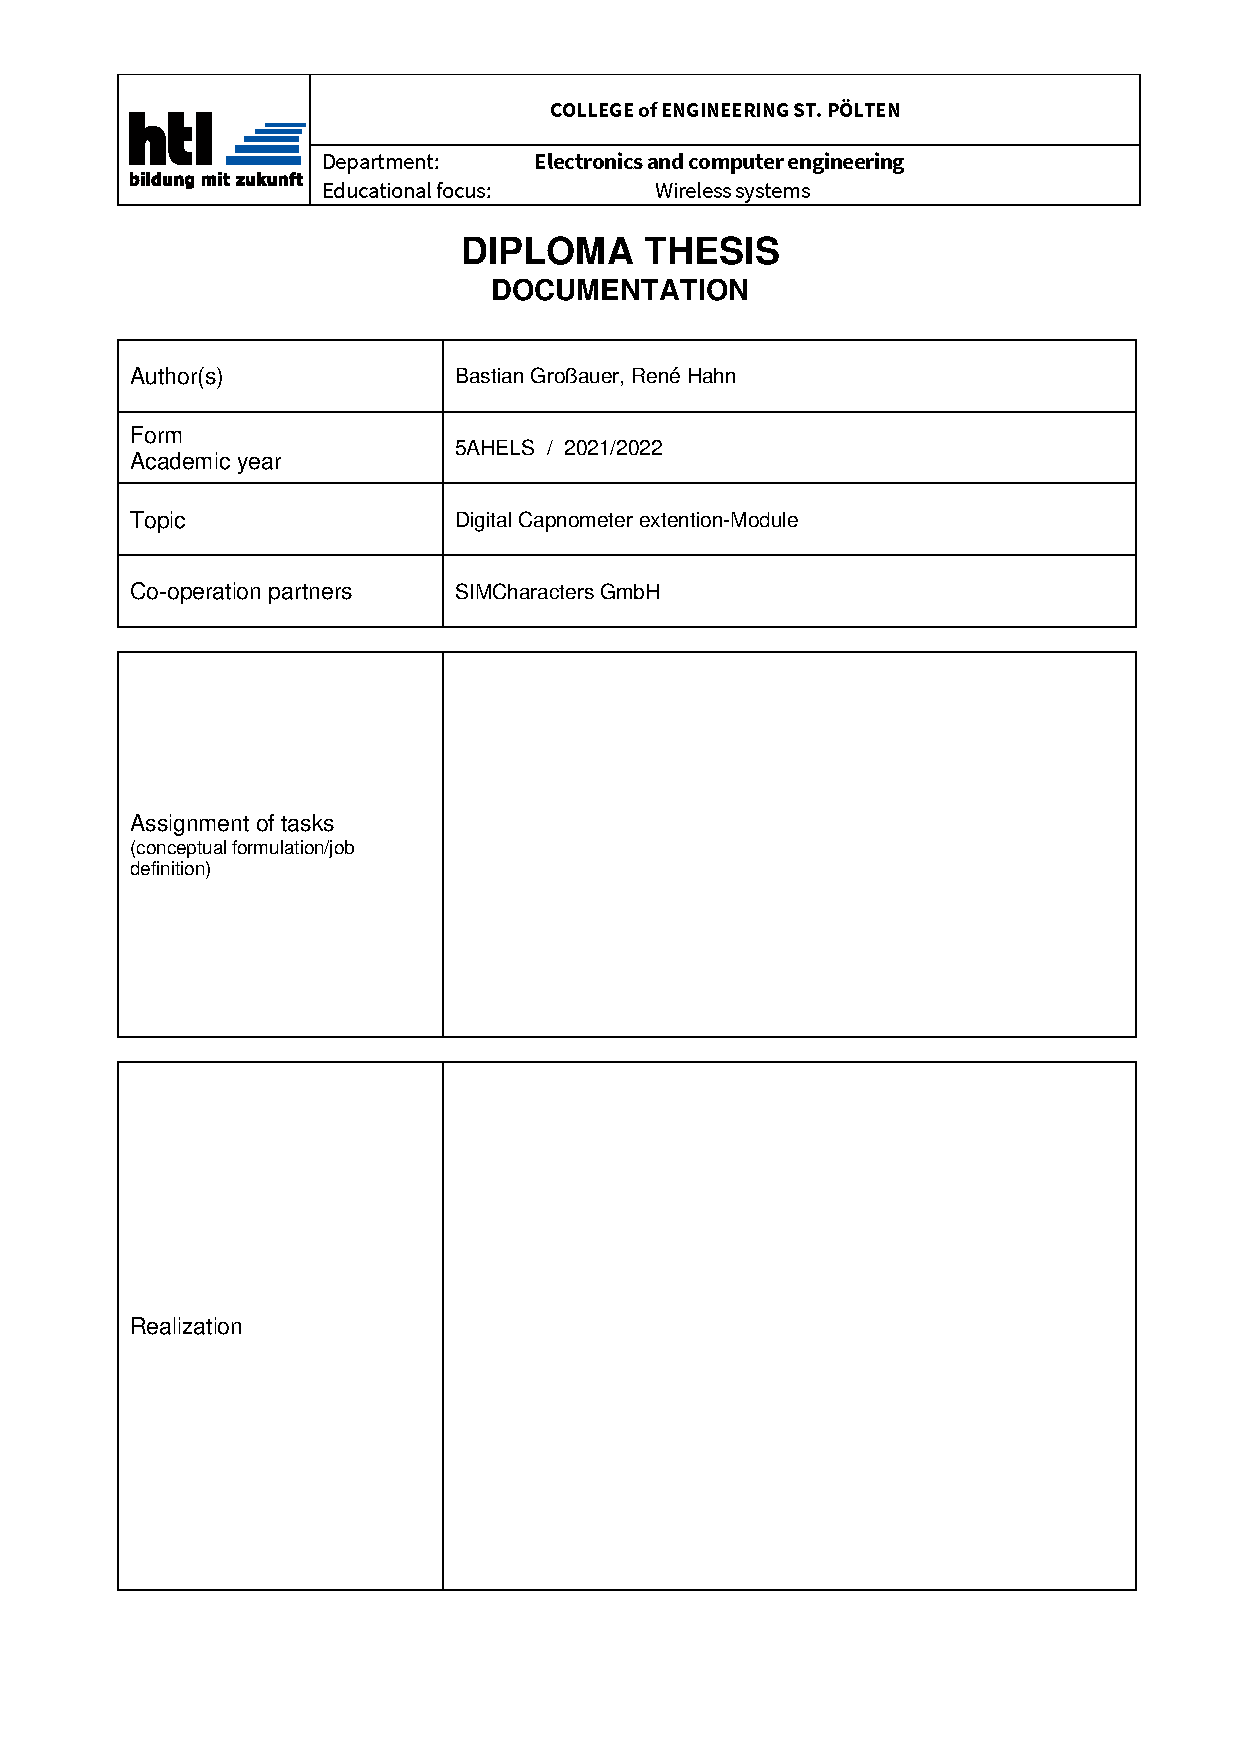
\includepdf[pages={1-2}]{./pdf/DA_3_CAPNO_nf.pdf}                                           % then export as pdf and add here

\clearpage                                                                                  % create an emty page
\thispagestyle{empty}
\hfill
\clearpage

\fancyhead{}
\clearpage


% --------------------------------------------- Acknoledgment -----------------------------------------------

\section*{Acknoledgement} 
\fancyfoot[RO,LE]{\thepage}   
\pagenumbering{Roman}                                                                       % set page count to roman numbers ONLY ON Table of content 
\setcounter{page}{1}

\fancyhead[RO,LE]{\textbf{Digital Capnometer Extension Module}\\\small{Acknoledgement}}     % change per new section


\par 
At this point, we would like to thank all the people, who helped and encouraged us throughout 
this entire diploma thesis. 

\par
....

\fancyfoot[C]{Bastian Großauer / René Hahn}


\clearpage


% ------------------------------------------- Table of Contents ---------------------------------------------

\fancyhead{}
\fancyhead[RO,LE]{\textbf{Digital Capnometer Extension Module}\\\small{Contents}}           % change small per new section
\fancyfoot[C]{}

\fancypagestyle{plain}{}
\tableofcontents                                                                       

% \clearpage                                                                                % If ToC ends on a right Page, Insert Blank Page
% \thispagestyle{empty}
% \hfill
% \clearpage

\cleardoublepage


% ----------------------------------------------- Preamble --------------------------------------------------

\setcounter{section}{-1}                                                                    % Set the Preamble to 0

\section{Preamble}
\setcounter{section}{0}
\fancyhead[RO,LE]{\textbf{Digital Capnometer Extension Module}\\\small{Preamble}}           % change per new section
\fancyfoot[RO,LE]{Page \thepage}    
\pagenumbering{arabic}                                                                      % set page count to roman numbers ONLY ON Table of content 
\setcounter{page}{1}

The overall goal of this ...

\fancyfoot[C]{Bastian Großauer}                                                             % change to who wrote that page, per page 


\cleardoublepage



% --------------------------------------------- Introduction ------------------------------------------------

\section{Introduction}
\fancyhead[RO,LE]{\textbf{Digital Capnometer Extension Module}\\\small{Introduction}}

\par 
I am the First Paragraphs

\par 
In this Diploma Thesis...

\begin{figure}[h]                                                                           % add a Picture; with [h] its after the last paragraph
    \centering
    
\includegraphics[scale=0.25]{./img/HTL.png}                                             % scales the Picture in %                                                              
    \caption{HTL Logo\cite{picture_HTL.png}}                                                    % add Picture (Link) and cite the Picture (only if its from an external source)
    \label{fig:figure1}                                                                     % add a Label for later references
\end{figure}

Lorem ipsum dolor sit amet, consetetur sadipscing elitr, sed diam nonumy eirmod tempor invidunt ut labore et dolore magna 
aliquyam erat, sed diam voluptua. At vero eos et accusam et justo duo dolores et ea rebum. Stet clita kasd gubergren, no 
sea takimata sanctus est Lorem ipsum dolor sit amet. Lorem ipsum dolor sit amet, consetetur sadipscing elitr, sed diam nonumy 
eirmod tempor invidunt ut labore et dolore magna aliquyam erat, sed diam voluptua. At vero eos et accusam et justo duo dolores 
et ea rebum. Stet clita kasd gubergren, no sea takimata sanctus est Lorem ipsum dolor sit amet. \cite{Lorem1}


\clearpage

\fancyfoot[C]{Bastian Großauer}                                                              % Add under every Page to display the writer 



\subsection{Subsection}

\par 
This is a Subsection



\subsubsection{Subsubsection}

\par
This is a Subsubsection

\para{Parapgraph} 

\par 
This is a SubSubSubSection also known as paragraph, one lower is subpara

\cleardoublepage                                                                              % Start Next Section with an odd Page (Right)


% --------------------------------------------- Specifications ------------------------------------------------

\section{Specifications}
\fancyhead[RO,LE]{\textbf{Digital Capnometer Extension Module}\\\small{Specifications}}




\fancyfoot[C]{Bastian Großauer}

\cleardoublepage


% ----------------------------------------------- Concept --------------------------------------------------

\section{Concept}

\fancyhead[RO,LE]{\textbf{Digital Capnometer Extension Module}\\\small{Concept}}



\fancyfoot[C]{Bastian Großauer}

\cleardoublepage

% ---------------------------------- Partition in Hardware and Software ------------------------------------

\section{Partition in Hardware and Software}
\fancyhead[RO,LE]{\textbf{Digital Capnometer Extension Module}\\\small{Partition in Hardware and Software}}

\fancyfoot[C]{Bastian Großauer}

\cleardoublepage


% --------------------------------------------- Used Technologies ------------------------------------------------

\section{Used Technologies}
\fancyhead[RO,LE]{\textbf{Digital Capnometer Extension Module}\\\small{Used Technologies}}



\fancyfoot[C]{Bastian Großauer}

\cleardoublepage

% --------------------------------------------- Research ------------------------------------------------

\section{Research}
\fancyhead[RO,LE]{\textbf{Digital Capnometer Extension Module}\\\small{Research}}


\fancyfoot[C]{Bastian Großauer}
\cleardoublepage


% ------------------------------------------ Hardware Design -------------------------------------------

\section{Hardware Design}
\fancyhead[RO,LE]{\textbf{Digital Capnometer Extension Module}\\\small{Hardware Design}}


\fancyfoot[C]{Bastian Großauer}

\cleardoublepage

% ------------------------------------------- Software Design -----------------------------------------------

\section{Software Design}
\fancyhead[RO,LE]{\textbf{Digital Capnometer Extension Module}\\\small{Software Design}}


\fancyfoot[C]{René Hahn}

\cleardoublepage


% ------------------------------------------------ Results ---------------------------------------------------
--

\section{Results}
\fancyhead[RO,LE]{\textbf{Digital Capnometer Extension Module}\\\small{Results}}


\fancyfoot[C]{Bastian Großauer}

\cleardoublepage


% --------------------------------------------- Economical Part ------------------------------------------------

\section{Economical Part}
\fancyhead[RO,LE]{\textbf{Digital Capnometer Extension Module}\\\small{Economical Part}}


\fancyfoot[C]{Bastian Großauer}

\cleardoublepage

% ------------------------------------------ Project Management ---------------------------------------------

\section{Project Management}
\fancyhead[RO,LE]{\textbf{Digital Capnometer Extension Module}\\\small{Project Management}}


\fancyfoot[C]{Bastian Großauer}

\cleardoublepage


% ----------------------------------------------- Appendix -------------------------------------------------
\appendix

\section{Appendix}
\fancyhead[RO,LE]{\textbf{Digital Capnometer Extension Module}\\\small{Appendix}}


\subsection{Milestones}

One part of project management is the milestone setting, because ...


\subsection{Internal Devision of Duties}

Bastian Großauer is in charge of the Hardware Design...

\subsection{Schedule}

The project was scheduled as ...


\subsection{Contact with the Projectpartner }

Initially, an email was sent to ...


\subsection{Diploma Seminars}

In the following pages the diploma seminars are visualized ...

\fancyfoot[C]{Bastian Großauer}


% Subsection Code Listings
\subsection{Code Listings}
\lstlistoflistings

% Subsection List of Figures
\subsection{List of Figures}
\listoffigures

% Subsection List of tables
\subsection{List of Tables}
\listoftables

%subsection 
\subsection{References}
\printbibliography[heading=none]


\end{document}
